\documentclass{article}
\usepackage[utf8]{inputenc}
\usepackage{graphicx}
\usepackage{amsmath}
\usepackage{amssymb}
\usepackage{subcaption}
\usepackage{float}

\title{Mat4 Aflevering 7}
\author{Roar Nind Steffensen}
\date{March 2016}

\begin{document}
\maketitle
\section*{Problem 5.11}

\begin{figure}[H]
    \centering
    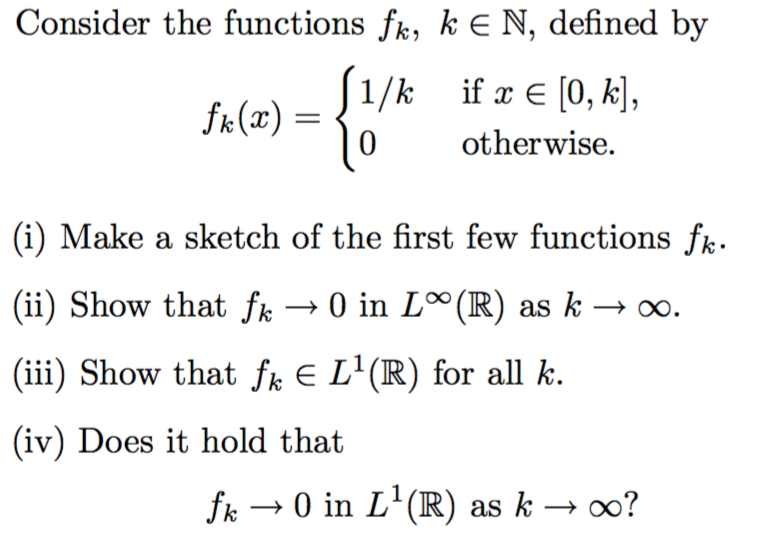
\includegraphics[width=7cm]{fig/prob511}
\end{figure}

\subsection*{Solution (i)}
\vspace{-5mm}
\begin{figure}[H]
 
\begin{subfigure}{0.45\textwidth}
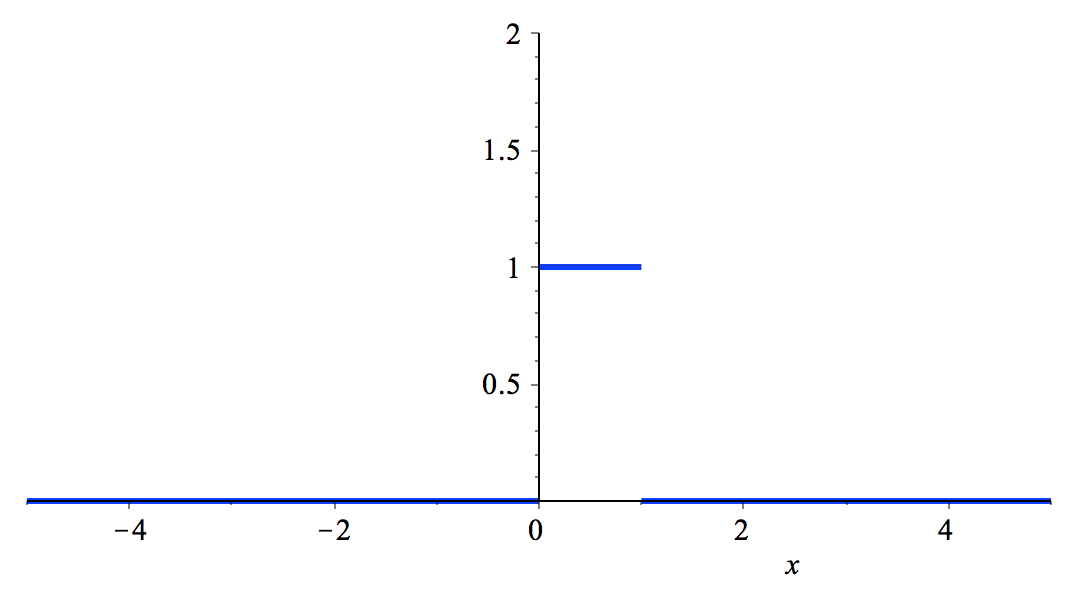
\includegraphics[width=0.9\linewidth, height=3cm]{fig/fk1} 
\caption{$f_1(x)$}
\end{subfigure}
\begin{subfigure}{0.45\textwidth}
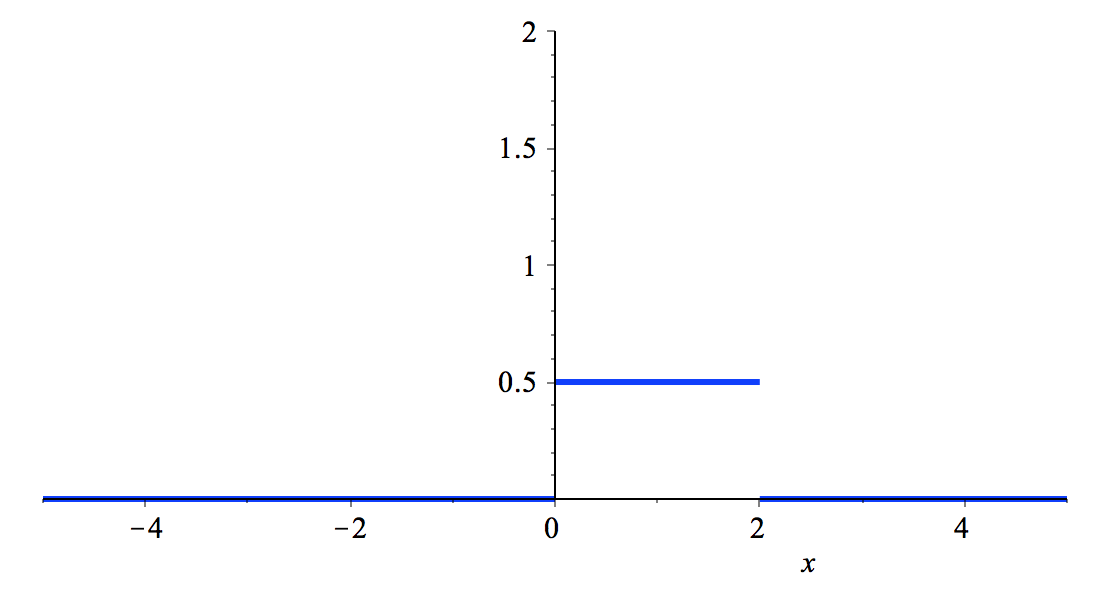
\includegraphics[width=0.9\linewidth, height=3cm]{fig/fk2}
\caption{$f_2(x)$}
\end{subfigure}
\begin{subfigure}{0.45\textwidth}
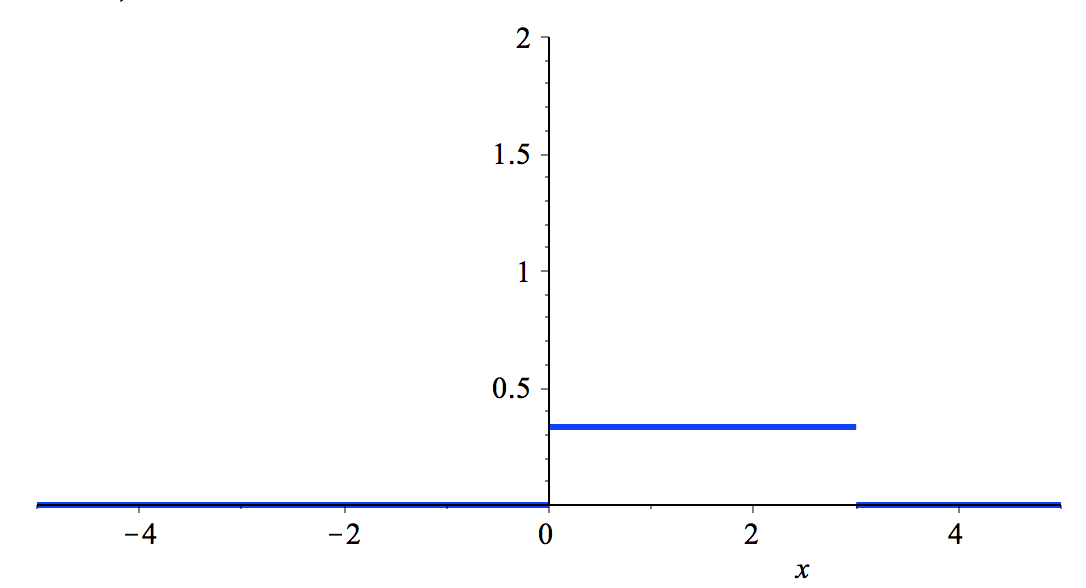
\includegraphics[width=0.9\linewidth, height=3cm]{fig/fk3} 
\caption{$f_3(x)$}
\end{subfigure}
\begin{subfigure}{0.45\textwidth}
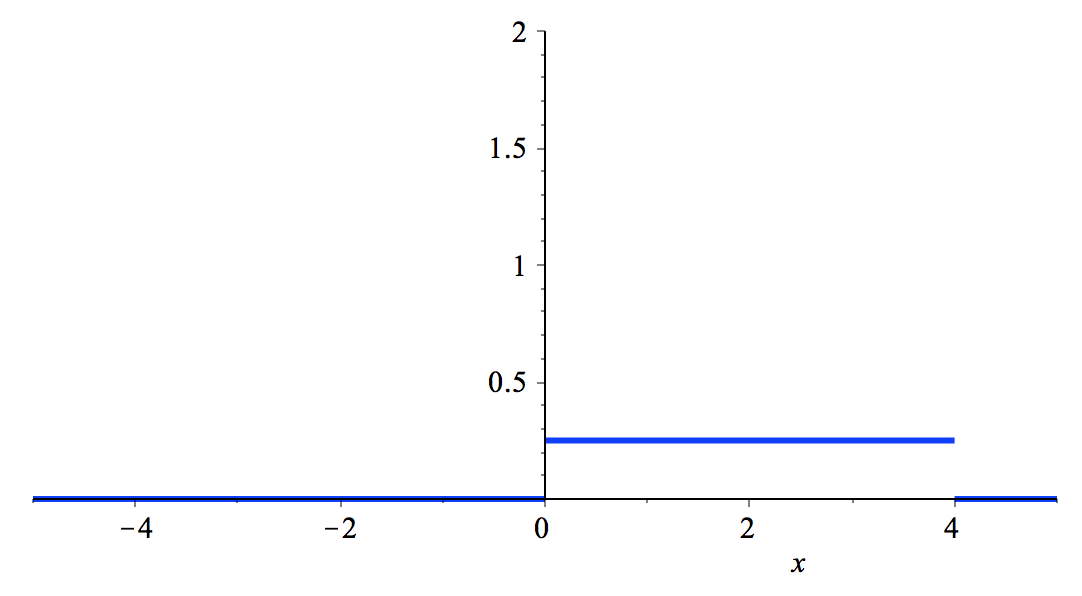
\includegraphics[width=0.9\linewidth, height=3cm]{fig/fk4}
\caption{$f_4(x)$}
\end{subfigure}
\end{figure}

\subsection*{Solution (ii)}

Assuming $f_k \in L^\infty(\mathbb{R})$, lets see what happens when $k\rightarrow \infty$. To do this, we use the norm, here being the supremums norm.

\begin{gather*}
    ||f_k||_\infty = \text{sup}\{|f_k(x)|\: | x \in \mathbb{R}\} = \frac{1}{k} \\
    \text{When} \: k \rightarrow \infty \Rightarrow \frac{1}{k} \rightarrow 0
\end{gather*}
Which leaves us with (from the definition of a norm) 
\begin{gather*}
     ||f_k||_\infty \rightarrow 0 \text{\: if \:} k \rightarrow \infty \Rightarrow \\
     f_k \rightarrow 0 \text{\: if \:} k \rightarrow \infty
\end{gather*}
On $L^\infty(\mathbb{R})$.

\subsection*{Solution (iii)}
For $f_k$ to be in $L^1(\mathbb{R})$ for all values of $k$ the norm must be finite. 
\begin{gather*}
    ||f_k||_1 = \int_{-\infty}^{\infty}|f_k(x)| \text{d}x = \frac{1}{k}k = 1
\end{gather*}
Which indeed is less than infinity, meaning that $f_k \in L^1(\mathbb{R})$ for all values of $k$.

\subsection*{Solution (iv)}
When $k \rightarrow \infty$ then $f_k(x) \rightarrow 0$ intuitively which would say that the statement holds. But from the norm, it states that $||f_k||_1 = 0 \Leftrightarrow f_k = 0$, for all functions identical \textit{almost} everywhere, which does not fulfil the statement. So it does not hold. 

\section*{Problem 4.28}
\begin{figure}[H]
    \centering
    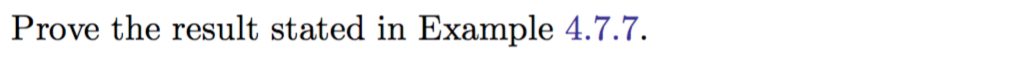
\includegraphics[width=10cm]{fig/prob428}
\end{figure}
\vspace{-8mm}
\begin{figure}[H]
    \centering
    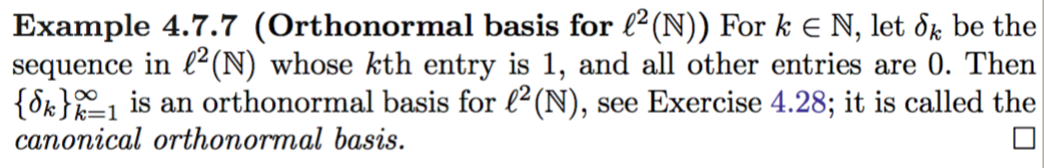
\includegraphics[width=10cm]{fig/ex477}
\end{figure}

\subsection*{Solution}
For the elements in $\{\delta_k\}_{k=1}^{}\infty$ to be orthonormal, we first check if they are orthogonal:
\begin{gather*}
    \delta_n \cdot \delta_m = \delta_{nm} = \left \{   \begin{tabular}{c}
  1 \text{\: if \:} n = m\\
  0 \text{\: if \:} n \neq m\\
  \end{tabular}
\end{gather*}

Which shows that they are orthogonal. Elementwise their length are 1, meaning they are orthonormal. To show that they are a basis for $l^2(\mathbb{N})$ we use the argumentation from example 3.2.2.\\

For $\{\delta_k\}_{k=1}^\infty$ to be a basis, it must hold, that for $u \in l^2(\mathbb{N}$ 

\begin{gather*}
    u = \sum_{k=1}^\infty c_k \delta_k
\end{gather*}
If $c_k$ is equivalent to the respective elements of $u$. This is written (using the norm) as

\begin{gather*}
   \left |\left | u - \sum_{k=1}^N c_k \delta_k\right | \right |_2 \rightarrow 0 \text{\:as\:}   N \rightarrow \infty 
\end{gather*}
We see that

\begin{gather*}
\left |\left | u - \sum_{k=1}^N c_k \delta_k\right | \right |_2 =\\
|| (u_1,u_2,...,u_N,u_{N+1},...)-(c_1,c_2,...,c_N,0,0...)||_2  = \\
|| (u_1-c_1,u_2-c_2,...,u_N-c_N,u_{N+1},...) ||_2 = \\
|| (u_{N+1},u_{N+2},...) ||_2 = \\
\left ( \sum_{k=N+1}^\infty \left | u_k \right |^2 \right)^{1/2}
\end{gather*}
And since $u \in l^2(\mathbb{N})$ we know that 
\begin{gather*}
    \left ( \sum_{k=1}^\infty \left | u_k \right |^2 \right)^{1/2} < \infty \Rightarrow \\
    \left |\left | u - \sum_{k=1}^N c_k \delta_k\right | \right |_2 = \left ( \sum_{k=N+1}^\infty \left | u_k \right |^2 \right)^{1/2} \rightarrow 0 \text{\: as \:} N \rightarrow \infty
\end{gather*}
Meaning that 
\begin{gather*}
    u = \sum_{k=1}^\infty c_k \delta_k
\end{gather*}
Proving that $\{\delta_k\}_{k=1}^\infty$ is a orthonormal basis for $l^2(\mathbb{N})$.

\section*{Problem 105}
\begin{figure}[H]
\centering
    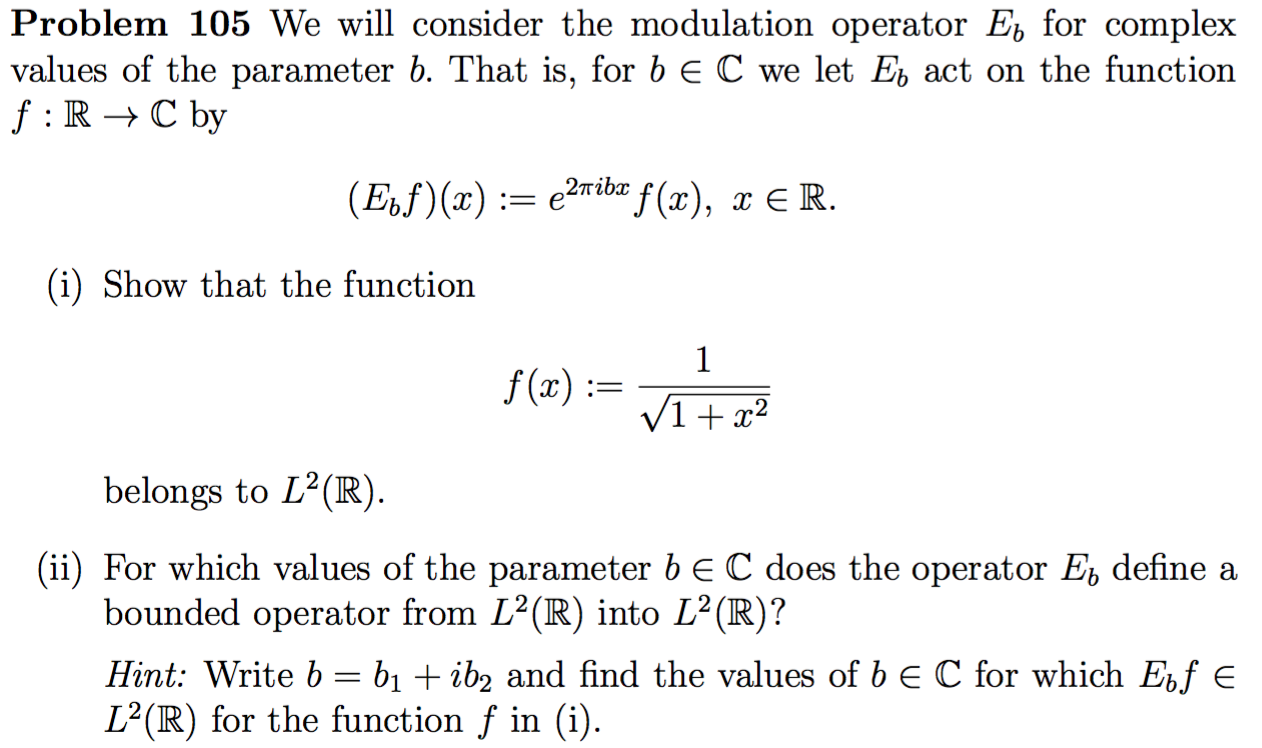
\includegraphics[width=10cm]{fig/prob105}
\end{figure}

\subsection*{Solution (i)}
To show that the function $f(x)$ is in $L^2(\mathbb{R})$ we show that the norm (for simplicity the norm squared) is finite.

\begin{gather*}
   \left( ||f||_2\right)^2=\int_{-\infty}^\infty \left |\frac{1}{\sqrt{1+x^2}}\right |^2 \text{d}x  = \\
    2\int_{0}^\infty \frac{1}{1+x^2} \text{d}x  =  2\left [\text{arctan(x)} \right]_0^\infty  = \pi
\end{gather*}
Which is finite, meaning that $f(x) \in L^2(\mathbb{R})$.

\subsection*{Solution (ii)}
In order to evaluate if the operator $E_b$ is bounded, it must first be well defined (again looking at the norm squared).

\begin{gather*}
    \left( ||E_b f||_2\right)^2 = \int_{-\infty}^\infty \left |e^{i 2 \pi b x}\frac{1}{1+x^2}\right |^2 \text{d}x = \int_{-\infty}^\infty \left(\left |e^{i 2 \pi b x}\right |\: \left |\frac{1}{1+x^2}\right |\right)^2 \text{d}x
\end{gather*}
Now if Im$(b)=0$ meaning that $b$ is real, this is solvable, otherwise if Im$(b)\neq 0$ this goes to infinity. Meaning that the operator is only defined on $L^2(\mathbb{R})$ if b is real which leaves us with
\begin{gather*}
     \int_{-\infty}^\infty \left(\left |e^{i 2 \pi b x}\right |\: \left |\frac{1}{1+x^2}\right |\right)^2 \text{d}x =  \int_{-\infty}^\infty \left(\lef \left |\frac{1}{1+x^2}\right |\right)^2 \text{d}x = \left( ||f||_2\right)^2
\end{gather*}

This also means that we have shown for what values of $b$ $E_b$ is a bounded operator. $E_b$ is a bounded operator on $L^2(\mathbb{R})$ when $b \in \mathbb{R}$ with $||T|| = 1$.

\end{document}
